\documentclass[11pt]{article}

\usepackage[review]{acl}

\usepackage{times}
\usepackage{latexsym}
\usepackage[T1]{fontenc}
\usepackage[utf8]{inputenc}
\usepackage{microtype}
\usepackage{inconsolata}
\usepackage{graphicx}
\usepackage{booktabs}
\usepackage{multirow}
\usepackage{amsmath}
\usepackage{amssymb}
\usepackage{tikz}
\usetikzlibrary{arrows.meta,positioning,calc,fit,backgrounds}
\usepackage{enumitem}
\usepackage{url}

% Compact leading, float and display spacing to fit the 8-page
% main-body limit.
\linespread{0.885}
\setlength{\textfloatsep}{8pt plus 2pt minus 2pt}
\setlength{\floatsep}{6pt plus 2pt minus 2pt}
\setlength{\intextsep}{6pt plus 2pt minus 2pt}
\setlength{\dbltextfloatsep}{8pt plus 2pt minus 2pt}
\setlength{\abovedisplayskip}{7pt plus 2pt minus 2pt}
\setlength{\belowdisplayskip}{7pt plus 2pt minus 2pt}
\setlength{\abovedisplayshortskip}{4pt plus 2pt minus 1pt}
\setlength{\belowdisplayshortskip}{4pt plus 2pt minus 1pt}

\title{Beyond Star Ratings: Weak Supervision and LLM-Assisted\\
Data Expansion for Chinese Review Sentiment Classification}

\author{Anonymous SRW Submission}

\begin{document}
\maketitle

\begin{abstract}
Chinese movie-review corpora provide abundant star ratings but few
semantic sentiment labels. Because ratings encode overall evaluation
rather than the polarity expressed in review text, they are an
imperfect supervision source for three-way sentiment classification.
We study how supervision source and data scale shape measured
performance through a weak-supervision pipeline seeded by 600
human-verified labels over a 910{,}998-review Douban corpus,
combining rating-derived signals, student pseudo-labels, and
uncertainty-sampled LLM annotations. On a 400-review,
identifier-disjoint human evaluation set, the 17K-label mixture
reaches 64.8\% accuracy versus 55.8\% for the deployed baseline and
55.75\% for a star-rating lookup (McNemar $p{<}0.01$). Star--text
agreement differs across review populations: 71.3\% on the
single-film seed set versus 55.8\% on the broader sample, and
three-star reviews are semantically neutral 30.6\% versus 56.8\% of
the time. Leakage ablations show that teacher-derived distillation
targets can materially affect fold-based performance estimates.
\end{abstract}

% Sections 1--3 of the NAACL 2027 SRW submission.
% Fragment only: no preamble, no \begin{document}.
% Requires: acl-style class, booktabs, and the bibliography keys cited below.

\section{Introduction}
\label{sec:intro}

Chinese movie-review corpora are abundant in ratings and impoverished
in labels. Douban attaches a five-star rating to every short review,
but review-level semantic sentiment labels---positive, neutral, or
negative as expressed in the text itself---are essentially absent at
scale. The two signals are not interchangeable: a rating records an
overall evaluation, often recommendation intent, whereas the text may
praise one aspect and attack another. Reviews are also terse (median
24 characters), frequently ironic, and dense with film-specific
allusion; mixed evaluations make even ``neutral'' contestable
\citep{pang2005seeing,zhang2018dl}.

This paper studies what it takes to learn three-class sentiment
classification under this label scarcity, organized around three
research questions. \textbf{RQ1}: How reliably do user star ratings
represent review-level semantic sentiment, and how does this vary
across review populations? \textbf{RQ2}: How does LLM-assisted data
expansion affect weakly-supervised Chinese review sentiment
classifiers? \textbf{RQ3}: How do supervision sources and evaluation
protocols influence measured performance?

Our setting is a 910{,}998-review Douban corpus derived from
Moviedata-10M \citep{moviedata10m}, carrying star ratings but no
semantic labels, anchored by \emph{gold-600}: 600 human-verified
semantic labels (592 unique texts) scraped from a single film page.
On this base we build a weakly-supervised pipeline in the tradition
of self-training and programmatic weak supervision
\citep{lee2013pseudo,xie2020selftraining,ratner2017snorkel}: the gold
anchor trains a teacher ensemble that labels the full corpus,
confidence-filtered pseudo-labels train corpus-scale specialists, and
uncertainty-guided active learning adds $\sim$17K rows labelled by a
mixture of LLM teachers and human adjudication \citep{settles2009}.
Because every supervision source carries a different provenance and
failure mode, we evaluate with a source-aware protocol: per-row
provenance splits, a row-level train/test contamination audit, and a
decomposition of the leakage channels that inflate naive out-of-fold
estimates.

Our findings qualify each link of this chain. Star ratings agree with
human semantic labels on only 71.3\% of gold-600, and the gap is
population-dependent: on a 400-review identifier-disjoint blind test
agreement falls to 55.75\%---only 30.6\% of three-star reviews are
semantic-neutral on gold-600 (56.8\% on the blind sample)---and a
pure star-rating lookup already matches our deployed ensemble
(55.75\% vs.\ 55.8\%). LLM-assisted expansion does help: a 17K-label
mixture improves on the deployed ensemble by 9.0pp on the blind human
test, though LLM-consensus labels inflate measured accuracy by
roughly 26 points relative to human-adjudicated rows. Supervision-
source provenance moves conclusions in both directions: 68.7\% of our
development benchmark's rows were exposed to earlier corpus-derived
training, and transitive corpus exposure, second-order teacher
targets, and duplicate texts account for most of the naive-vs-corrected
OOF gap ($\sim$7pp three-class, $\sim$4pp binary; corrected figures
82.6--83.1\% / 91.5\%).

We make three contributions:
\begin{itemize}
  \item \textbf{An empirical analysis of the rating--sentiment gap}
        across three review populations (a curated single-film gold
        set, an identifier-disjoint blind human test, and the
        weakly-labelled corpus), locating where star supervision fails
        and how much a star-lookup baseline already explains.
  \item \textbf{A scalable weakly-supervised pipeline} combining
        star-derived weak labels, student pseudo-labels, and
        uncertainty-guided LLM annotation ($\sim$17K added labels),
        improving on the deployed ensemble by 9.0pp on
        identifier-disjoint human labels.
  \item \textbf{A source-aware evaluation protocol} for
        weakly-supervised pipelines---provenance-split reporting,
        row-level contamination audits, and leakage decomposition---
        that moves measured performance by several points.
\end{itemize}
Section~\ref{sec:related} reviews related work;
Section~\ref{sec:data} describes the datasets and annotation protocols;
Sections~\ref{sec:method}--\ref{sec:results} present the pipeline,
setup, and results; Section~\ref{sec:limitations} states limitations.

\section{Related Work}
\label{sec:related}

\subsection{Weakly Supervised Text Classification}

Learning from noisy or programmatic labels is mature: Snorkel
\citep{ratner2017snorkel} formalised weak supervision through
labelling functions; self-training \citep{lee2013pseudo} and its
noisy-student descendant \citep{xie2020selftraining}, extended by
consistency-training variants such as UDA \citep{xie2020uda}, show
that confident predictions can bootstrap larger training sets;
uncertainty-driven sampling underlies active learning
\citep{settles2009}; and loss correction \citep{arazo2021pseudo} and
confident learning \citep{northcutt2021} characterise which examples
are likely mislabeled. This literature treats label noise as a
property of the \emph{training} signal and reports on a fixed
evaluation split; we instead measure each supervision source's noise
structure directly (RQ1) and audit the evaluation itself (RQ3).

\subsection{LLM-Assisted Data Annotation}

LLM annotation is increasingly common: zero-shot LLMs can rival or
exceed crowd workers \citep{gilardi2023}, but two cautions apply.
First, LLM suggestions anchor human annotators toward model
predictions \citep{schroeder2025humanloop}; our adjudication
interface displayed the student model's prediction and confidence,
so our 479 human-adjudicated rows are explicitly exposed to this
effect (Section~\ref{sec:data}). Second, two passes of the
\emph{same} LLM share inductive bias rather than providing
independent annotation, and models trained on LLM-augmented data
inherit teacher conventions \citep{moller2024parrot}; on subjective
tasks annotator disagreement is informative rather than noise
\citep{davani2022}. We therefore treat LLM two-pass consensus as a
pseudo-label source, never ground truth \citep{zenimoto2024,neveditsin2025}.

\subsection{Review Sentiment Analysis}

Review sentiment analysis ranges from early work establishing that
star ratings and review polarity are related but distinct signals
\citep{pang2005seeing} through opinion-mining surveys
\citep{pang2008opinion} and deep models \citep{zhang2018dl}. Chinese
review sentiment relies on pre-trained encoders---MacBERT
\citep{cui2020macbert} and sentiment-enhanced SKEP
\citep{tian2020skep} are our backbone choices---and aspect-level
models for mixed evaluations \citep{wang2016attention}. Prior work
assumes text-level labels exist; we ask how far star ratings,
pseudo-labels, and LLM labels can substitute for them.

\subsection{Evaluation and Dataset Quality}

Data contamination in evaluation is increasingly documented for LLM
benchmarks, with taxonomies distinguishing incidental from targeted
exposure \citep{sainz2023contamination,balloccu2024}, and leakage is
a recognised reproducibility hazard \citep{kapoor2023}. For OOD
evaluation, classical detection baselines \citep{hendrycks2017} and
benchmarks such as \citet{baran2023ood} establish protocols we
adapt; reusing a development set for model selection introduces
measurable optimism \citep{cawley2010}; and
\citet{dror2018hitchhiker} provide the statistical-testing
discipline---McNemar tests, bootstrap intervals, Holm
correction---that we apply to every comparison. Reporting norms for
human evaluation and annotation \citep{kunilovskaya2026,alkhalifa2026}
and dataset documentation \citep{bender2018,gebru2021} motivate our
per-row provenance fields; unlike audits of released benchmarks
\citep{toossi2024}, we audit a pipeline we build ourselves.

\section{Dataset and Annotation}
\label{sec:data}

\subsection{Overview}

The task is three-class sentiment classification
$y \in \{\text{positive}, \text{neutral}, \text{negative}\}$ of Douban
movie short reviews. Corpus reviews are short (median 24 characters)
and frequently contain sarcasm, film-specific allusions, or mixed
polarity, so the neutral class is both frequent and ambiguous.
Table~\ref{tab:datasets} summarises every dataset, its annotation
source, and its role. Two properties are unusual and deliberate:
several ``test'' sets carry LLM-generated labels, and one of them
(ood1000) is a \emph{development/selection} set, not a held-out test.

\begin{table}[t]
\centering
\scriptsize
\setlength{\tabcolsep}{2pt}
\caption{Datasets and annotation sources. ``Consensus'' = agreement of
two blind LLM passes; ``adjudicated'' = human resolution of pass
disagreements plus spot-checked agreements. Roles reflect the audited,
corrected protocol. The $\sim$17K AL pools mix 279 human-adjudicated,
721 consensus, and $\sim$15.9K DeepSeek-V4.1-Flash teacher labels;
their text-level audit is in Appendix~\ref{app:human400}.}
\label{tab:datasets}
\begin{tabular}{@{}p{1.5cm}r p{2.9cm} p{1.6cm}@{}}
\toprule
Dataset & Rows & Annotation source & Role \\
\midrule
gold-600 & 600 & Human semantic labels; star-rule weak labels & Train anchor; OOF eval \\
pseudo pools & 910{,}998 & Star-rating rule; student pseudo-labels & Weak supervision \\
ood1000 & 1{,}000 & 800 LLM consensus + 200 human-adjudicated & Dev/selection set \\
al1000 & 1{,}000 & 721 LLM consensus + 279 human-adjudicated & AL training \\
AL expansions (al5000--al17k) & $\sim$17{,}000 & 279 human-adj.; 721 consensus; $\sim$15.9K DS-Flash teacher & AL training \\
fresh500 & 500 & DeepSeek-V4.1-Flash zero-shot labels & Dev replication check (partially exposed) \\
lab500 & 500 & Two LLM annotators; 331 consensus rows & Superseded pilot; partially exposed \\
human-400 & 400 & Blind single-annotator labels; length-stratified & Identifier-disjoint, single-annotator, length-stratified human test \\
\bottomrule
\end{tabular}
\end{table}

\subsection{Gold-600: human labels and the star-rating gap}

The gold set was scraped from the first 30 pages of a single Douban
movie page: 600 rows covering 592 unique reviews (316 positive / 92
neutral / 192 negative). Eight exact-duplicate text pairs were
\emph{not} removed before training or evaluation, so duplicates can
land in different cross-validation folds---a residual fold-isolation
violation analysed in Appendix~\ref{app:audit}. Each row carries two
labels: \texttt{label\_rule}, a star-derived three-class weak label,
and \texttt{label\_semantic}, a human-verified semantic label.
Fourteen rows lack a star rating and are excluded from rating-derived
supervision and the agreement analysis below; neutral-class decision
rules (Appendix~\ref{app:annotation}) are applied consistently across
gold, adjudication, and human-400 labelling. Reviews here are longer
than corpus reviews ($\sim$111 vs.\ 40 characters), and neutral rests
on only 92 examples. All 600 texts were sent to Alibaba PAI for a
baseline comparison; we disclose this egress in
Section~\ref{sec:limitations}.

The dual labels let us measure, rather than assume, star ratings as
sentiment supervision. On the 586 gold rows carrying both labels,
per-star agreement is 94.3\% (1$\star$), 85.9\% (2$\star$),
\textbf{30.6\%} (3$\star$), 78.7\% (4$\star$), and 96.9\% (5$\star$);
overall agreement is \textbf{71.3\%}. The failure is concentrated in
the middle band---51.3\% of three-star reviews are semantically
\emph{negative}, not neutral---so we use ratings only as weak
pretraining signal, never as gold labels.

\subsection{Weakly-labelled corpus}

The weak corpus derives from Moviedata-10M \citep{moviedata10m}: 4.43M
raw Douban comments cleaned and deduplicated to \textbf{910{,}998}
reviews spanning 20{,}966 films and 249{,}105 users, with star rating,
timestamp, and vote counts but no semantic labels. It is the source of
all pseudo-label pools: a student ensemble labels the full corpus, a
confidence-filtered subset (271{,}905 rows at $p \ge 0.7$) trains
corpus-scale specialists, and margin/entropy sampling selects the
active-learning pools below.

\subsection{LLM-assisted benchmarks: lab2000 and successors}

\paragraph{lab2000.} To measure---and then narrow---the
gold-to-corpus generalisation gap, we built \textbf{lab2000}: 2{,}000
corpus reviews in two disjoint subsets. \textbf{ood1000} samples
1{,}000 reviews uniformly at random (gold-deduplicated, cross-movie)
and served as the development benchmark for model selection.
\textbf{al1000} samples 1{,}000 reviews by margin/entropy sampling
from the deployed student's predictions---deliberately the hardest
rows---and is a training set, not a test set. Active-learning expansion
continued through al5000, al5000b, and disagreement-mined al3k rounds,
producing pools up to $\sim$17K rows of mixed provenance (279
human-adjudicated, 721 same-LLM-agent consensus, $\sim$15.9K
DeepSeek-V4.1-Flash teacher labels, plus a Qwen3-4B ablation); all AL
pools are verified text-disjoint from every evaluation set.

\paragraph{Annotation protocol.} Each lab2000 row was labelled twice by
two independent inference passes of the \emph{same} LLM annotator model
with different few-shot example sets, blind to star ratings and to each
other's output---single-model self-consistency, not two independent
annotators. Inter-pass agreement was 86.7\% ($\kappa=0.80$) on ood1000
and 79.8\% ($\kappa=0.67$) on al1000; the lower agreement on the
margin-selected set is itself evidence that AL mining selects
intrinsically ambiguous rows. All 335 inter-pass disagreements plus 144
spot-checked agreements were adjudicated by the author, yielding
\textbf{479 human-adjudicated rows} (200 in ood1000, 279 in al1000);
the remaining rows take two-pass consensus (Table~\ref{tab:datasets}).

\paragraph{fresh500 and lab500.} \textbf{fresh500}: 500 uniformly
sampled corpus reviews labelled zero-shot by DeepSeek-V4.1-Flash; our
audit finds zero text overlap with the gold/AL pools but 70.2\% of its
rows share a corpus identifier with earlier corpus-derived training,
so it is a replication check on a partially exposed distribution, not
a clean test. \textbf{lab500} (superseded pilot): 500 reviews labelled
by two LLM annotators with 331 consensus rows; a pilot CV script used
lab500 itself for training, so it is partially exposed.

\paragraph{human-400.} Our identifier-disjoint final test: 400 corpus
reviews sampled with length stratification (160/120/80/40 across
$\le$20, 21--50, 51--100, and $>$100 characters) after excluding
every previously used identifier pool, and blind-labelled by one
author under written guidelines (Appendix~\ref{app:annotation}).
Post-hoc audits verify zero comment-ID overlap with every training
pool of every evaluated system, and a text-level audit against
462{,}879 pool texts (Appendix~\ref{app:human400}) finds zero exact
or near-duplicate overlap plus only two ultra-short boilerplate
normalized matches in corpus pseudo-label pools. The
length-stratified sample is benchmark-specific, not a population
estimate; labels are positive 156 / neutral 179 / negative 65.
Star-implied labels agree with these human labels on only
\textbf{55.75\%} of rows (vs.\ 71.3\% on gold-600); among 5$\star$
reviews only 62.7\% are semantically positive. Single-annotator
labelling means no IAA is computable; we treat human-400 as our
primary OOD evidence while flagging the limitation in
Section~\ref{sec:limitations}.

\subsection{Annotation quality: what the agreement numbers do and do not show}

We report agreement following standard IAA practice
\citep{artstein2008} and the reporting norms of
\citeauthor{kunilovskaya2026} (\citeyear{kunilovskaya2026}) and
\citeauthor{alkhalifa2026} (\citeyear{alkhalifa2026}); dataset
documentation follows data-statement and datasheet conventions
\citep{bender2018,gebru2021} (Appendix~\ref{app:ethics}). Three
caveats qualify all agreement numbers below. First, a 200-row random
subset of ood1000 was blind-labelled by a second human annotator, but
because the released labels mix 47 human-adjudicated and 153
LLM-consensus rows, the measured 71.5\% raw / $\kappa=0.568$ (95\% CI
$[0.47,0.66]$) is a human-vs-\emph{reference} figure, not a pure
human--human IAA. Second, on the 47 adjudicated rows where both LLM
passes and the human label are available, the two passes agree on only
\textbf{29.8\%} ($\kappa=-0.18$) versus 86.7\% overall---consensus
labels are least reliable on exactly the hard rows that decide
rankings. Third, adjudication displayed the deployed student's
prediction and confidence, the anchoring setting of
\citeauthor{schroeder2025humanloop} (\citeyear{schroeder2025humanloop});
our 479 ``human'' labels may be biased toward stu3c-family outputs,
which matters because the same family produces the pseudo-labels being
evaluated; Sections \ref{sec:method}--\ref{sec:results} quantify each.

%% draft_sections_4_5.tex — NAACL 2027 SRW fragment (Sections 4--5)
%% \input this file into paper/srw.tex in place of the three % TODO blocks.
%% Figure labels fig:pipeline / fig:al-scaling are placeholders pending the
%% final figure files (blueprint: Fig 1 = pipeline+data flow, Fig 2 = AL
%% scaling curve or label-provenance distribution).

\section{Methodology}
\label{sec:method}

\subsection{System overview}
\label{sec:method:system}

Our deployed system is a two-channel ensemble over Chinese review text
(Figure~\ref{fig:pipeline}). The \emph{student} channel is a
\emph{hfl/chinese-macbert-base} classifier \citep{cui2020macbert}; the
\emph{judge} channel is a small MLP head on frozen
MegatronBERT-1.3B features. Both channels emit class-probability
vectors $P_s$ and $P_j$, blended with fixed weights $1{:}2$:
\begin{equation}
  \mathrm{dep} \;=\; \tfrac{1}{3}\,P_s \;+\; \tfrac{2}{3}\,P_j .
  \label{eq:dep}
\end{equation}
For the three-class task, a \emph{neutral probability correction
module} refines $\mathrm{dep}$. The module is deliberately not an
independent three-way classifier: it estimates only
$P(\mathrm{neutral})$ and leaves the positive/negative split to
$\mathrm{dep}$. Two estimators of $P(\mathrm{neu})$---a frozen-feature
MLP head and a corpus-trained neutral detector---are mixed as
$p_n = 0.6\,P_{\mathrm{neu}}^{\mathrm{head}} +
0.4\,P_{\mathrm{neu}}^{\mathrm{corpus}}$. Writing $r_{+}, r_{-}$ for the
positive/negative masses of $\mathrm{dep}$ renormalized to sum to one, the
corrected distribution and final blend are
\begin{equation}
  \begin{aligned}
    \mathrm{corr} &= \big[(1-p_n)\,r_{+},\; p_n,\; (1-p_n)\,r_{-}\big],\\
    \mathrm{final} &= \frac{\mathrm{dep} + 0.5\,\mathrm{corr}}{1.5}.
  \end{aligned}
  \label{eq:spec}
\end{equation}
We adopt this targeted correction rather than simpler alternatives:
class weighting, decision-threshold adjustment, focal loss, and
class-balanced oversampling were evaluated and rejected
(Appendix~\ref{app:negative}). Its macro-F1 gain over the
uncorrected blend is positive but not statistically significant
(McNemar $p{=}0.65$; bootstrap 95\% CI $[-0.4,+3.8]$pp;
\S\ref{sec:res-ablations}), so we treat the module as a neutral-recall
repair whose benefit must be re-verified on human400
(\S\ref{sec:res-human400}).

A single post-hoc temperature $T{=}0.37$ calibrates the three-class
probabilities; it is fitted by NLL on the same gold-600 OOF
predictions---in-sample calibration---and is argmax-invariant, so it
affects neither accuracy nor macro-F1. For ultra-short slang-only
inputs, an exact-match lexicon guard overrides the ensemble before
inference (verified conflict-free on gold-600). The binary task uses
the same dep-blend without the correction module and a fixed 0.5
decision threshold.

\begin{figure}[t]
\centering
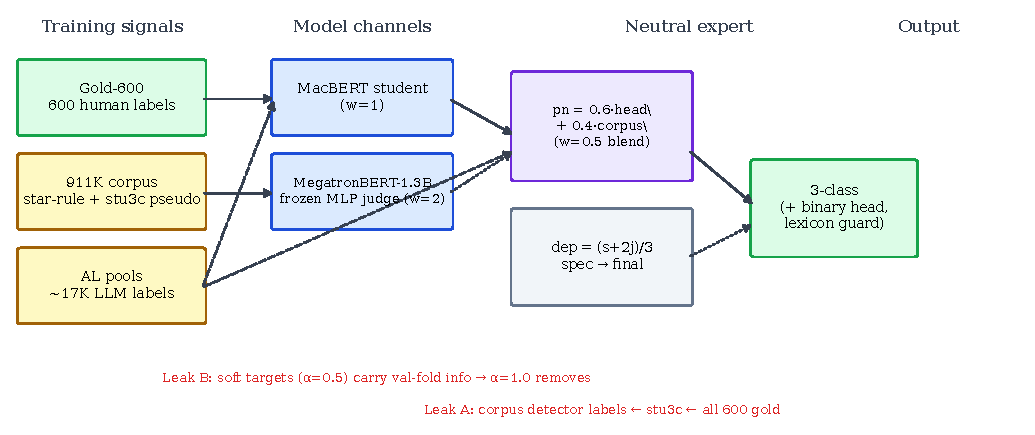
\includegraphics[width=\columnwidth]{fig1_pipeline.pdf}
\caption{Deployed three-class pipeline and its training-signal chain.
Leak~A: the corpus neutral detector's labels descend from stu3c, a
student fit on all 600 gold rows, so its gold predictions carry
whole-set information. Leak~B: distillation soft targets
($\alpha{=}0.5$) are produced by teacher channels whose folds overlap
the student's validation fold. The $\alpha{=}1.0$ ablation removes the
teacher term; the corpus-channel toggle bounds Leak~A.}
\label{fig:pipeline}
\end{figure}

\subsection{Training signal chain}
\label{sec:method:chain}

Labels reach the deployed models through four stages, each of which later
proved relevant to our audit.

\paragraph{Gold seed.} 600 human semantic labels from a single Douban
film page (316 positive / 92 neutral / 192 negative; binary evaluation
on the 508 non-neutral rows) provide hard and soft targets for the
first students and judges.

\paragraph{Distillation objective.} The gold-trained students and the
frozen-feature judge heads are optimized with a mixed hard/soft
objective \citep{hinton2015distilling} rather than plain
cross-entropy: for a training row $i$ with hard label $y_i$ and
teacher probability vector $q_i$ (the deployed teacher ensemble's
stored out-of-fold prediction for that row), the per-sample loss is
{\small
\begin{equation}
  \begin{aligned}
  \ell_i = {}& \alpha\,\mathrm{CE}(z_i, y_i) \\
             & +\; (1-\alpha)\,\tau^{2}\,
  \mathrm{KL}\!\Big(\mathrm{softmax}\big(q_i/\tau\big)\,\Big\|\,
  \mathrm{softmax}\big(z_i/\tau\big)\Big),
  \end{aligned}
  \label{eq:kd}
\end{equation}
}
where $z_i$ are the student's logits, $\mathrm{CE}$ is (optionally
class-weighted) cross-entropy, and the second term is standard
temperature-scaled distillation: both $q_i$ and $z_i$ are divided by
$\tau{=}2$ before the softmax, and the teacher$\,\|\,$student KL
divergence summed over classes is rescaled by $\tau^{2}$. Crucially,
$\alpha$ weights the \emph{hard}-label term, not the teacher term:
$\alpha{=}0.5$ gives hard labels and teacher soft targets equal
weight, while $\alpha{=}1.0$ sets the teacher weight to exactly zero
and recovers pure hard-label training (the same objective trains the
MLP judge heads). Teacher probabilities are fixed per-row vectors
from the deployed teacher ensembles, and teacher and student share
the same 5-fold partition, so the KD term on a student's training
rows is not independent of its validation fold (Leak~B,
\S\ref{sec:audit}); the $\alpha{=}1.0$ ablation removes the teacher
term entirely while holding folds, hyperparameters, and fusion
weights fixed.

\paragraph{Pseudo-label pools.} Following classical self-training and
pseudo-labeling practice \citep{lee2013pseudo,xie2020selftraining}, a
3-class student re-scores all 910{,}998 corpus rows under a
weak-supervision framework \citep{ratner2017snorkel}; the confident
pool ($\mathrm{conf}{\ge}0.7$, 271{,}905 rows) is sampled under
per-class caps into 115K--195K-row training subsets for full-fit
corpus-trained models. Binary pools use $\mathrm{conf}{\ge}0.8$;
star-rating-derived label variants serve as ablations.

\paragraph{Corpus-trained models.} Full-fit MacBERT students and
frozen-feature MLP heads are trained on these pseudo-label pools,
including the deployed neutral corpus detector.

\paragraph{Active learning and SFT mixes.} Margin-band
($[0.15,0.70)$) and cross-student disagreement mining select 17{,}000
mutually disjoint corpus rows, labeled by LLM teachers (DeepSeek-V4.1-Flash
primary; Qwen3-4B and hybrid variants as comparisons) in rounds from
1K to 17K labels. A per-fold SFT student is trained on gold$+$AL
labels and fused with the deployed ensemble at weight $w_{\mathrm{SFT}}$
selected by 5-fold cross-validation.

\subsection{Audit methodology}
\label{sec:audit}

Alongside the system we contribute a source-aware evaluation
protocol, distinguishing three levels of evaluation independence---
\emph{per-row fold isolation}, \emph{upstream signal isolation}, and
\emph{selection independence}---of which our headline score satisfied
only the first, up to eight exact-duplicate gold-600 texts that can
cross stratified folds (Appendix~\ref{app:audit} gives the taxonomy).
Two leak mechanisms violate upstream signal isolation.
\textbf{Leak~A} (transitive pseudo-label): a channel's training labels
are outputs of a model fit on 100\% of the evaluation labels---the
chain gold$\to$stu3c$\to$911K pseudo-labels$\to$corpus detector places
gold information inside the deployed neutral channel at $\approx$13\%
effective weight. \textbf{Leak~B} (second-order teacher): per-fold
soft distillation targets (Eq.~\ref{eq:kd}) are emitted by teachers
whose own folds overlap the student's validation fold, so at
$\alpha{=}0.5$ the teacher-KD term carries half the loss weight and
half the distillation signal is second-order. Both are invisible to
standard OOF reporting because the CV machinery itself is correct.

Our \emph{leak-isolation protocol} reruns all distilled channels with
$\alpha{=}1.0$ (pure hard-label cross-entropy) holding folds,
hyperparameters, and fusion weights fixed, and toggles the corpus
channel on/off. A \emph{row-level cid audit} intersects every
evaluation set's comment IDs with each corpus-derived model's training
manifest, reporting per-model and union overlap plus near-duplicates.
A \emph{selection-bias accounting} enumerates the full candidate pool
(26 mixtures, $\approx$73 SFT runs), reports every number as a maximum
over it, and distinguishes cross-fit from oracle selection
\citep{dror2018hitchhiker}. All OOD numbers are reported \emph{split
by annotation provenance}.

\section{Experimental Setup}
\label{sec:setup}

\paragraph{Evaluation sets.} Table~1 (\S\ref{sec:data}) inventories all
label sources; here we fix the \emph{role} of each set under the audit.
\textbf{gold-600 OOF} was never used for Stage-2 OOD model selection,
but deployed v3's configuration and fusion weights were tuned on
gold-600 itself, so its OOF estimates are not fully selection-
independent (frozen tuned weights, Leak~A/B bounded by the
$\alpha{=}1.0$ ablation, eight exact-duplicate texts able to cross
folds); corrected estimates therefore also rerun all distilled
channels on the deduplicated \textbf{gold-592} set under identical
ungrouped folds (Appendix~\ref{app:audit}). \textbf{ood1000}
($n{=}1000$; 800 LLM-consensus + 200 human-adjudicated, the latter
labelled with student predictions visible) is the
\emph{development/selection set} for every Stage-2 decision, not a
held-out test. \textbf{fresh500} has zero text overlap with gold/AL
pools but $\sim$70\% comment-ID overlap with corpus-derived training,
DeepSeek-Flash labels from the same teacher family as $\approx$16K AL
labels, and only the top-2 ood1000 configurations evaluated---a
replication check on a partially exposed distribution. \textbf{lab500}
is a superseded, row-level contaminated pilot. \textbf{human400}
($n{=}400$) is our identifier-disjoint final test: length-stratified,
blind single-author labels, zero comment-ID overlap verified
post-hoc, and a text-level audit finding 0 exact, 0 near-duplicate,
and 2 normalized boilerplate matches against all evaluated systems'
training pools (Appendices~\ref{app:annotation}, \ref{app:human400}).

\paragraph{Metrics, systems, implementation.} We report accuracy and
macro-F1 for both tasks, plus per-class recall to expose neutral-class
collapse; comparisons use McNemar's exact test, 5{,}000-resample
bootstrap confidence intervals, and Holm correction over the
22-test comparison family \citep{dror2018hitchhiker}. Systems compared:
deployed v3 (uncorrected and $\alpha{=}1.0$ ablations); SFT mixtures
at AL scales 1K--17K; TF-IDF and frozen-feature MLP baselines;
Qwen3-4B zero-shot; DeepSeek-V4.1-Flash and V4-Pro zero-shot teachers.
MacBERT-base student; frozen MegatronBERT-1.3B judge head (shared
backbone feature pass); 5-fold \texttt{StratifiedKFold} (seed 42, no
group constraints) for gold OOF, reapplied identically to the 592
unique texts for the deduplicated rerun, and seed-0 cross-fit for
mixture weights; seeds \{42, 123, 456, 789, 999\}; max length 256;
distillation $\alpha\in\{0.5,1.0\}$, $\tau{=}2$, 8 epochs for students
and 300 epochs for MLP heads. The deployed three-class system
additionally requires the frozen 1.3B-parameter judge backbone (and
the corpus neutral detector) at inference; only the student channel
is compact enough for edge deployment. Full hyperparameters are
released with the code and configuration log.

%% draft_sections_6.tex — NAACL 2027 SRW fragment (Section 6)
%% Restructured 2026-07: results lead with research findings (rating--sentiment,
%% AL scaling, human400 generalization), followed by provenance/evaluation
%% sensitivity and ablations. Labels sec:res-ablations / sec:res-human400 are
%% referenced from draft_4_5 and must be kept.
\section{Results and Analysis}
\label{sec:results}

\subsection{Rating--Sentiment Divergence Across Review Populations}
\label{sec:res-rating}

Star ratings are the cheapest supervision signal in our corpus, so we
first measure what they actually encode. gold-600 carries dual labels:
a star-implied class and a human semantic label. On the 586 rows
carrying both, agreement is only \textbf{71.3\%}, and the failure is
concentrated in the middle band---just \textbf{30.6\%} of three-star
reviews are semantic-neutral, while 51.3\% are semantically
\emph{negative}. Ratings are informative at the extremes (94--97\%
agreement at 1$\star$ and 5$\star$) and unreliable at 3$\star$.

The divergence is \emph{population-dependent}, the central finding of
this analysis. Replicating the same star-rule comparison on
human400---our identifier-disjoint, blind-labelled sample---drops
agreement to \textbf{55.75\%} (223/400) and \emph{reverses} the
three-star pattern: 56.8\% of human400 three-star reviews are
semantic-neutral (versus 30.6\% on gold-600), while 4$\star$ agreement
falls from 78.7\% to 50.7\%. The curated single-film gold set
over-represents negative-leaning mid-range raters; a random corpus
sample does not. At corpus scale the same gap appears without human
labels: student pseudo-labels agree with the star-implied class on
only 47.8\% of all 910{,}998 reviews (54.0\% inside the confident
pool).

The practical consequence is immediate: a pure star-rating lookup
scores exactly 223/400 $=$ 55.75\% on human400---statistically
indistinguishable from our deployed ensemble's 55.8\%
(\S\ref{sec:res-human400}). Ratings therefore serve only as weak
pretraining signal; semantic labels must come from humans or LLM
teachers, which motivates the expansion studied next
(\S\ref{sec:res-al}).

\subsection{Scaling Weak Supervision with LLM-Assisted Annotation}
\label{sec:res-al}

We expand supervision along the two axes of \S\ref{sec:method:chain}:
margin-band and cross-student-disagreement mining select corpus rows
for LLM annotation, and the resulting $\sim$17K-row AL pools (279
human-adjudicated, 721 LLM-consensus, $\sim$15.9K DeepSeek-V4.1-Flash
teacher labels) train a per-fold SFT student fused with the deployed
ensemble at weight $w_{\mathrm{SFT}}$ chosen by cross-validation.

Figure~\ref{fig:al-scaling} plots three-class accuracy on the ood1000
\emph{development} set as the AL pool grows: gold$+$al1000 starts at
72.0\%, the 6K hybrid-teacher pool reaches 74.2\%, the 11K DeepSeek
pool 74.9\%, the 14K pool 75.5\%, and the 17K pool \textbf{77.1\%}
(5-seed average, macro-F1 77.4)---versus deployed v3's 65.0\%. The SFT
student alone reaches 74.1\%, so most of the gain survives without
fusion. Two controls qualify the curve: disagreement-mined selection
alone (al3kds, 3K rows) reaches only 71.5\%, below the larger 6K pool
(scale, not selection cleverness, drives the gain); and teacher
provenance matters at fixed size---the Qwen3-4B-teacher 11K variant
reaches 72.4\% versus 74.9\% for DeepSeek, while an all-DeepSeek 11K
variant dropping the adjudicated core (al11kds0) is statistically
indistinguishable (75.2\% vs.\ 74.9\%, McNemar $p{=}0.81$), consistent
with the label-convention alignment of \S\ref{sec:res-provenance}.
Binary mixtures follow the same trend, peaking at 92.3\%/92.0\%
(accuracy/macro-F1, $n{=}673$ non-neutral).

All of these are development-set estimates subject to the selection
accounting of \S\ref{sec:res-provenance}; the decisive test is
human400, where the frozen al17k recipe---weights selected on ood1000,
never re-tuned---reaches \textbf{64.8\%}, $+9.0$pp over v3
(\S\ref{sec:res-human400}).

\begin{figure}[t]
\centering
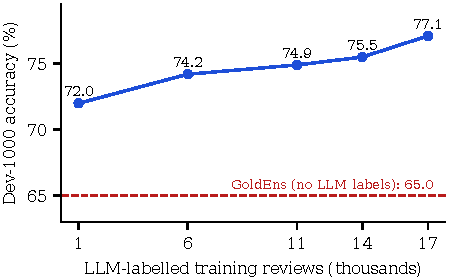
\includegraphics[width=0.85\columnwidth]{fig3_al_scaling.pdf}
\caption{Three-class accuracy on the ood1000 development set versus
AL pool size for the SFT$+$v3 mixture (DeepSeek/hybrid teachers;
1K $=$ gold$+$al1000). The curve is monotone but every point is a
best-of-$N$ development estimate (\S\ref{sec:res-provenance}).}
\label{fig:al-scaling}
\end{figure}

\subsection{Generalization on Human-Labeled Reviews: human400}
\label{sec:res-human400}

human400 is the only evaluation set in this paper with \emph{zero
known identifier overlap} with any training pool and fully human
labels: 400 corpus reviews, length-stratified (160/120/80/40),
identifier-excluded and blind-labelled by a single author
(\S\ref{sec:data}; Appendices~\ref{app:annotation}, \ref{app:human400}).
Labels: 156~positive / 179~neutral / 65~negative; single-annotator,
so no human--human IAA is available, and the stratified sample is a
benchmark, not a population estimate. A text-level overlap audit
(exact, normalized, near-duplicate) found zero exact or
near-duplicate overlap with the pools of evaluated systems and only
two ultra-short normalized matches in corpus pseudo-label pools
(Appendix~\ref{app:human400}).

On it, deployed v3 reaches 55.8\% three-class accuracy (macro-F1
55.4) and 76.5\% binary accuracy on the 221 non-neutral rows---far
below its dev-set estimates and exactly matched by the star-rating
lookup of \S\ref{sec:res-rating} (223/400 $=$ 55.75\%; per-rating,
only 62.7\% of 5-star and 50.7\% of 4-star reviews are labelled
positive by the annotator).

The frozen-weight al17k mixture reaches \textbf{64.8\%} three-class
accuracy (macro-F1 63.5), $+9.0$pp over both v3 and the star lookup.
The gain is real but its significance is concentrated: raw McNemar
tests give $p{=}1.3{\times}10^{-3}$ versus v3 and $7.4{\times}10^{-3}$
versus the star lookup; under Holm correction over the 16 pairwise
human400 comparisons (Appendix~\ref{app:human400}) only the
mix-vs-v3 result survives (adjusted $p{=}0.021$; mix-vs-star
adjusted $p{=}0.104$). This \emph{reverses} the teacher-alignment
worry: on identifier-disjoint human labels the AL gains are genuine
generalization over the deployed system, though the margin over a
rating baseline is nominally, not family-wise, significant.
Per-class, the gain is a neutral-class repair: neutral F1
rises 55.9$\to$68.0 (recall 50.3$\to$73.7) while negative recall
drops 81.5$\to$66.2 in exchange for much higher negative precision
(35.3$\to$54.4); full per-class precision/recall/F1 for all five
systems is in Appendix~\ref{app:human400}
(Table~\ref{tab:human400-perclass}). Caveats: accuracy on
annotator-flagged \emph{mixed} reviews drops below v3 (40.0\% vs.\
53.3\%, $n{=}30$); Qwen3-4B zero-shot reaches 61.5\%/59.0, below the
mixture (raw McNemar $p{=}0.26$).

Binary ($n{=}221$): v3 reaches 76.5\%, below the rating rule (83.7\%),
which the frozen mixture \emph{matches exactly} (83.7\%) while
predicting a more balanced class distribution and a higher macro-F1
(81.3 vs.\ 77.9). The two make identical numbers of errors in
opposite directions (28/28 symmetric discordance, $p{=}1.0$), so the
binary gain over the rating rule is class balance, not accuracy;
versus v3 the raw McNemar $p{=}0.020$ does not survive Holm correction
(adjusted $p{=}0.234$; Appendix~\ref{app:human400}).

\subsection{Annotation Provenance and Evaluation Sensitivity}
\label{sec:res-provenance}

Every number in this paper means something different depending on
where its labels came from and how the model was selected: leakage-
channel ablations on the gold OOF estimates, the development-set
status and provenance of ood1000, and row-level train/test
contamination.

\paragraph{Gold-OOF leakage decomposition.}
Table~\ref{tab:main-results} contrasts our previously reported
(uncorrected) headline with the leakage-reduced $\alpha{=}1.0$ rerun.
The three-class deployed 89.5\%/85.9\% decomposes cleanly: Leak~B
(second-order teacher targets) accounts for $+5.5$pp accuracy
($89.5\to84.0$ with the corpus channel kept), and the transitive
corpus channel (Leak~A) contributes a further $+0.7$pp that vanishes
when removed ($84.0\to83.3$), leaving a leakage-reduced OOF range of
\textbf{83.3--84.0\% accuracy / 76.3--77.8 macro-F1} (the deduplicated
rerun reported with the ablations gives 82.6--83.1\%). The binary
pipeline has no corpus channel, so its entire inflation ($+3.0$pp) is
Leak~B, leaving \textbf{92.9\%/92.4\%} (91.5\%/90.8 deduplicated).
These are leakage-channel ablation estimates, not a fully nested,
selection-independent final-system score (single seed, frozen weights
tuned on gold-600, $\alpha{=}1.0$ not re-tuned, residual
duplicate-text channel; \S\ref{sec:res-ablations}). Our earlier
headline claims were inflated; the honest numbers are the
contribution.

\begin{table}[t]
\centering
\scriptsize
\begin{tabular*}{\columnwidth}{@{\extracolsep{\fill}}lp{3.5cm}cc@{}}
\toprule
Task & Pipeline variant & Acc & Macro-F1 \\
\midrule
\multirow{4}{*}{3-class}
 & deployed, uncorrected ($\alpha{=}0.5$) & 89.5 & 85.9 \\
 & $\alpha{=}1.0$, corpus kept & 84.0 & 77.8 \\
 & $\alpha{=}1.0$, corpus removed & 83.3 & 76.3 \\
 & $\alpha{=}0.5$, corpus removed & 87.5 & 81.3 \\
\midrule
\multirow{2}{*}{binary}
 & deployed, uncorrected ($\alpha{=}0.5$) & 95.9 & 95.6 \\
 & $\alpha{=}1.0$ (no corpus channel) & 92.9 & 92.4 \\
\bottomrule
\end{tabular*}
\caption{Gold-600 out-of-fold results (\%). ``Uncorrected'' rows are the
previously reported deployed scores; $\alpha{=}1.0$ rows remove second-order
teacher leakage (Leak~B). The corpus-channel toggle bounds Leak~A.
Leak~B $\approx{+}5.5$pp (3-class) / ${+}3.0$pp (binary); Leak~A
$\approx{+}0.7$pp.}
\label{tab:main-results}
\end{table}

\paragraph{ood1000 is a development set.} Every Stage-2 decision was
read off ood1000 accuracy: AL scale (1K$\to$17K), teacher choice
(DeepSeek/Qwen/hybrid), per-task epochs, seed count and subset, and
fusion weights via cross-validation on ood1000 itself---26 mixture
configurations and $\approx$73 SFT runs in total. OOD claims are only
as honest as the selection protocol behind them \citep{baran2023ood};
we therefore report ood1000 numbers as \emph{development estimates}
with an estimated best-of-$N$ optimism of $+0.3$--$1.0$pp (3-class)
and $+0.2$--$0.7$pp (binary), and McNemar tests on this set are
anti-conservative because it was reused for selection.

\paragraph{Row-level contamination.} Our cid audit
(Appendix~\ref{app:audit}) shows evaluation texts entered corpus
training sets: 68.7\% of ood1000, 70.2\% of fresh500, and 74.8\% of
lab500 rows share a corpus ID with at least one corpus-trained model,
plus 220/107 near-duplicate rows on ood/fresh; the deployed neutral
detector trained on 13.0\%/13.2\% of ood1000/fresh500. AL/SFT pools
have \emph{zero} cid overlap, so SFT-mix gains cannot be explained by
row memorization, but every corpus-channel number carries bounded
exposure.

\paragraph{Label provenance splits the benchmark.}
Table~\ref{tab:ood-results} splits ood1000 by label provenance. Every
system drops 20--32pp on the 200 human-adjudicated rows---though this
gap confounds label source with item difficulty, since the adjudicated
rows are exactly the disagreement-enriched, harder items. On this
subset the ranking changes: DeepSeek-V4.1-Flash zero-shot (59.5\%,
$n{=}195$ parseable) \emph{exceeds} our best local mixture (56.0\%),
while v3 falls to 46.5\%. The two LLM passes agree on only 29.8\% of
the 47 adjudicated rows ($\kappa{=}{-}0.18$) versus 100\% on consensus
rows by construction, indicating consensus labels encode a single
model's conventions \citep{schroeder2025humanloop,moller2024parrot}
---part of the mixture's consensus-subset lead is label-convention
alignment, not broad generalization. Binary is more robust: the best
mix loses only 8.4pp across provenance (93.7$\to$85.3) versus 26.4pp
three-class.

\paragraph{fresh500 is a partially exposed replication.}
On \textbf{fresh500}---zero text overlap with gold/AL pools but
$\sim$70\% comment-ID overlap with corpus-derived training and
DeepSeek-Flash labels from the same teacher family as $\approx$16K AL
labels---the fixed al17k recipe replicates at 77.0\%/93.7\% versus
v3's 58.8\%/86.3\%, but it measures agreement with teacher
conventions as much as generalization, and only the top-2 ood1000
configurations were evaluated on it.

\begin{table}[t]
\centering\scriptsize
\setlength{\tabcolsep}{2.5pt}
\begin{tabular}{llcccc}
\toprule
Eval rows & $n$ & v3 & al17kds mix & DS-Flash & Qwen3-4B \\
\midrule
ood1000, all (dev) & 1000 & 65.0 & 77.1 & 82.0 & 70.6 \\
\quad LLM-consensus & 800 & 69.6 & 82.4 & 87.5 & 75.1 \\
\quad human-adjudicated & 200 & 46.5 & 56.0 & 59.5 & 52.5 \\
\midrule
fresh500 (DS labels) & 500 & 58.8 & 77.0 & --- & --- \\
\midrule
human400 (blind human) & 400 & 55.8 & 64.8 & --- & 61.5 \\
\bottomrule
\end{tabular}
\caption{3-class accuracy (\%) by evaluation set and label provenance.
ood1000 is a development/selection set; its 200 adjudicated rows were
labelled with student predictions visible, and the consensus-vs-
adjudicated gap confounds label source with item difficulty
(\S\ref{sec:res-provenance}). DS-Flash is scored on its parseable rows
only: $n{=}992/797/195$ of the 1000/800/200 rows above; all other
columns use every row. human400 labels are single-author blind
annotations on an identifier-disjoint, length-stratified sample; mix
uses frozen ood1000-selected weights (\S\ref{sec:res-human400}).}
\label{tab:ood-results}
\end{table}

\subsection{Model Ablations and Error Analysis}
\label{sec:res-ablations}

\paragraph{Duplicate-text leakage.} A further channel affects even the
$\alpha{=}1.0$ estimates: gold-600 has 600 rows but only 592 unique
texts---8 exact-duplicate pairs (Appendix~\ref{app:audit})---and every
OOF script uses stratified $k$-fold without group constraints, so
duplicates can cross folds (expected $\approx$6--7 of 8 pairs),
violating per-fold isolation; we estimate the inflation at $\sim$1--2pp,
concentrated in neutral/negative classes. Retraining the full pipeline
on the 592 unique texts with dedup-aligned teachers moves the
$\alpha{=}1.0$ estimates to \textbf{82.6--83.1\%} three-class /
74.8--75.9 macro-F1 and \textbf{91.5\%} / 90.8 binary (from 83.3--84.0
/ 76.3--77.8 and 92.9 / 92.4 on the 600 rows); the $\alpha{=}0.5$
variant drops more (86.5\% vs.\ 89.5\%). These deduplicated
leakage-reduced OOF estimates are the in-domain numbers we stand behind.

\paragraph{Diagnostics and negative results.}
Appendix~\ref{app:ablations} collects the statistical diagnostics:
adjacent AL scales are within noise (al17kds\_avg5 vs.\
al14kds\_avg: $+1.6$pp, McNemar $p{=}0.064$); the v2$\to$v3
neutral-correction gain is positive but non-significant
($\Delta$macro-F1 $+1.6$pp; bootstrap 95\% CI $[-0.4,+3.8]$pp;
McNemar $p{=}0.65$); the OOD drop is \emph{not} a short-text artifact
(neutral recall collapses 51.1$\to$33.3\% across ood1000 length
buckets); and IAA is $\kappa{=}0.568$ against a \emph{blended}
human/LLM reference only. Over twenty variants were rejected
(Appendix~\ref{app:negative}); headline selection thus operated on
ood1000, and a fold-isolated corpus detector, re-tuned fusion weights,
and a second human400 annotator would further change our conclusions.


\section{Conclusion}
\label{sec:conclusion}

We set out to scale semantic sentiment classification for Chinese
Douban reviews under weak supervision, and the empirical picture that
emerged is threefold. First, star ratings are an informative but
unreliable semantic proxy whose meaning shifts across populations:
rating--text agreement is 71.3\% on the single-film gold-600 seed set
but only 55.8\% on the broader human400 sample, and the three-star
band flips from majority negative (30.6\% neutral) on gold-600 to
majority neutral (56.8\%) on human400. Second, uncertainty-guided LLM
data expansion yields genuine generalization: on the
identifier-disjoint human400 test the frozen-weight 17K mixture
reaches 64.8\% three-class accuracy, $+9.0$pp over deployed v3
(McNemar $p{=}1.3{\times}10^{-3}$), while a star-rating lookup
matching v3 shows how little signal the ratings alone carry. Third,
supervision provenance shapes measured performance: teacher-derived
distillation targets inflated fold-based OOF estimates by
$\approx$5.5pp, ood1000 functioned as a development set rather than a
held-out test, and LLM-consensus labels overstated accuracy by
$\approx$26 points relative to human-adjudicated rows. These results
argue for provenance-aware evaluation whenever weak or
model-generated labels feed either training or benchmarking. Future
work includes fold-isolated corpus channels, fusion weights re-tuned
on leakage-free signals, a second annotator for human400, and
multi-annotator protocols for LLM-assisted benchmark construction.

\section{Limitations}
\label{sec:limitations}

Several boundary conditions scope our claims. gold-600 is drawn from
a single film page, so in-domain numbers are not cross-domain
estimates, and its 600 rows retain eight exact-duplicate text pairs
that can cross CV folds (Appendix~\ref{app:audit}). human400 is
length-stratified (160/120/80/40) and single-annotator, so its
results are benchmark-specific rather than population estimates; its
text-level overlap audit against all training pools is reported in
Appendix~\ref{app:human400}. Identifier-disjointness removes known
training-pool exposure but does not prove contamination-free text:
the audit found two ultra-short boilerplate normalized matches in
corpus pseudo-label pools feeding one ensemble channel.
The 479 adjudicated rows were labelled with student predictions
visible, likely anchoring labels toward model outputs; ood1000 was
used for model selection and has substantial identifier overlap, so
its figures are selection-conditioned development estimates and its
McNemar tests are anti-conservative; and our human--reference
agreement ($\kappa{=}0.57$) blends human and same-LLM-consensus
references, so it is not a pure human--human IAA. The corrected OOF
figures (83.3--84.0\% three-class / 92.9\% binary on the 600 rows;
82.6--83.1\% / 91.5\% after deduplication) are single-seed,
frozen-weight leakage-channel ablation estimates still subject to
fusion-weight selection bias, not fully selection-independent
final-system scores. Finally, all 600 gold texts were processed on a
commercial training platform (Alibaba Cloud PAI) for a baseline
comparison; this egress is disclosed in Section~\ref{sec:ethics}.

\section{Ethical Considerations}
\label{sec:ethics}

All review texts are Douban user comments used without platform
authorization: the gold-600 set was scraped from a single film page
and the corpus derives from the Moviedata-10M release, whose terms
prohibit redistribution of raw texts. We therefore release labels,
identifiers and SHA-256 text hashes rather than review text; users
may re-join source texts under the upstream license. Roughly 18.5K
unique texts were transmitted to the DeepSeek API for teacher
labelling and all 600 gold texts were processed on Alibaba Cloud
PAI; only review text and star ratings were sent, with no direct
identifiers. DeepSeek's published privacy policy permits the
provider to use de-identified inputs and outputs for service
improvement; no zero-retention agreement was in place, and API
data is stored in the People's Republic of China. Annotation was
performed by the authors and one additional annotator on publicly
posted, non-sensitive film reviews; users were not contacted, and
the task involved no human-subjects experimentation beyond the
annotators' own labeling of public posts.
A fuller ethics statement and data-availability details appear in
Appendix~\ref{app:ethics}.

\bibliography{refs}

% Appendix (unlimited pages). Terminology matches body.tex:
%   GoldEns = gold-only ensemble; Gold-600 student = its MacBERT component fitted on
%   all 600 rows; LLM-17K = 16,906 LLM-labelled corpus reviews; Dev-1000 = uniform
%   development sample; Human-400 = blind human test; Fresh-500 = uniform sample with
%   DeepSeek labels. File and script names in \texttt keep their repository spelling.

\appendix

\section{GoldEns: Architecture and Training}
\label{app:goldens}

GoldEns is a two-channel ensemble. The \emph{student} channel is a
\emph{hfl/chinese-macbert-base} classifier \citep{cui2020macbert}; the
\emph{judge} channel is an MLP head on frozen features of
Erlangshen-MegatronBERT-1.3B-Sentiment \citep{fengshenbang2022}. With
class-probability vectors $P_s$ and $P_j$,
\begin{equation}
  \mathrm{dep} \;=\; \tfrac{1}{3}\,P_s \;+\; \tfrac{2}{3}\,P_j .
  \label{eq:dep}
\end{equation}
For the three-way task a neutral-probability correction refines
$\mathrm{dep}$. It estimates only $P(\text{neutral})$ and leaves the
positive/negative split to $\mathrm{dep}$. Two estimators, a
frozen-feature MLP head and a MacBERT neutral detector trained on
115{,}000 corpus pseudo-labels from the Gold-600 student, are mixed
as $p_n = 0.6\,P_{\mathrm{neu}}^{\mathrm{head}} +
0.4\,P_{\mathrm{neu}}^{\mathrm{corpus}}$. Writing $r_{+}, r_{-}$ for
the positive and negative masses of $\mathrm{dep}$ renormalised to
sum to one,
\begin{equation}
  \begin{aligned}
    \mathrm{corr} &= \big[(1-p_n)\,r_{+},\; p_n,\; (1-p_n)\,r_{-}\big],\\
    \mathrm{final} &= \frac{\mathrm{dep} + 0.5\,\mathrm{corr}}{1.5}.
  \end{aligned}
  \label{eq:spec}
\end{equation}
On Gold-600 the correction raises out-of-fold macro-F1 by 1.6 points
over the uncorrected blend, a gain that is not significant (McNemar
$p{=}0.65$; bootstrap 95\% CI $[-0.4,+3.8]$ points). The binary task
uses the blend of Eq.~\ref{eq:dep} with dedicated binary models and a
0.5 threshold. A post-hoc temperature ($T{=}0.37$, fitted on the same
out-of-fold predictions) reduces expected calibration error from
0.251 to about 0.04 in-sample and does not change any prediction.

\paragraph{Distillation objective.}
The gold-trained student and judge heads are trained with a mixed
hard/soft objective \citep{hinton2015distilling}. For a training row
$i$ with hard label $y_i$, student logits $z_i$ and a teacher
probability vector $q_i$ (the stored out-of-fold prediction of a
larger gold-trained ensemble),
{\small
\begin{equation}
  \begin{aligned}
  \ell_i = {}& \alpha\,\mathrm{CE}(z_i, y_i) \\
             & +\; (1-\alpha)\,\tau^{2}\,
  \mathrm{KL}\!\Big(\mathrm{softmax}\big(q_i/\tau\big)\,\Big\|\,
  \mathrm{softmax}\big(z_i/\tau\big)\Big),
  \end{aligned}
  \label{eq:kd}
\end{equation}
}%
with $\tau{=}2$. The weight $\alpha$ applies to the hard-label term:
$\alpha{=}0.5$ is the configuration first evaluated, and
$\alpha{=}1.0$ removes the teacher term entirely.

\paragraph{Hyperparameters.}
Students: 8 epochs, maximum length 256, seed 42. MLP heads: 300
epochs. Cross-validation: five-fold \texttt{StratifiedKFold} (seed
42, no group constraint), reapplied to the 592 unique texts for the
deduplicated rerun. LLM-label student: seeds \{42, 123, 456, 789,
999\} for the three-way model (4 epochs) and \{42, 123, 789, 999\} for
the binary model (8 epochs). At inference GoldEns needs the frozen
1.3B-parameter backbone; the LLM-label student is a single
MacBERT-base model.

\section{Evaluation Provenance and Leakage}
\label{app:audit}

This appendix supports \S\ref{sec:res-provenance}.

\subsection{Three levels of independence}
We distinguish (i) \emph{per-row fold isolation}: each evaluation row
was absent from the training fold of every model that scored it;
(ii) \emph{upstream signal isolation}: no artifact whose construction
used the evaluation row's label feeds a model that scores it; and
(iii) \emph{selection independence}: no hyperparameter, weight or
checkpoint was chosen on the evaluation set. The 89.5\% figure for
GoldEns satisfied (i) only approximately and failed (ii) and (iii).

\paragraph{Teacher targets (Leak B).}
Every distilled model was trained with soft targets
($\alpha{=}0.5$) from teacher ensembles whose predictions on the
student's validation fold came from models trained on that fold;
teacher and student share one fold assignment. Retraining all three
tasks with $\alpha{=}1.0$ and rebuilding the pipeline with folds,
hyperparameters and fusion weights fixed lowers three-way accuracy
from 89.5\% to 84.0\% (macro-F1 85.9 to 77.8) and binary accuracy
from 95.9\% to 92.9\% (macro-F1 95.6 to 92.4). Fusion weights were
not re-tuned, so the corrected figures are conservative.

\paragraph{Pseudo-label detector (Leak A).}
The neutral detector was trained on 115{,}000 corpus pseudo-labels
produced by the Gold-600 student, a model fitted to all 600 gold
rows. Its scores on gold rows therefore carry information about every
gold label, not only those of its own fold; its stored gold
probabilities equal that student's elementwise. The detector
contributes about 13\% of the output mass ($0.4 \times 0.5/1.5$).
Removing it changes three-way accuracy from 84.0\% to 83.3\%
(macro-F1 77.8 to 76.3).

\paragraph{Duplicate texts.}
Gold-600 has 600 rows but 592 unique texts: eight exact-duplicate
pairs that were not removed before training or evaluation. With
ungrouped stratified folds, six to seven of the eight pairs are
expected to be split across folds. Retraining on the 592 unique texts
with deduplicated teachers moves the $\alpha{=}1.0$ estimates to
82.6--83.1\% three-way (macro-F1 74.8--75.9) and 91.5\% binary
(macro-F1 90.8); the $\alpha{=}0.5$ variant falls to 86.5\%.

\paragraph{Selection on Dev-1000.}
The LLM-label study iterated on Dev-1000: pool size (1K to 17K),
teacher (DeepSeek, Qwen, hybrid), epochs, seed subsets and fusion
weights were all compared there, the last by five-fold cross-fitting
on Dev-1000 itself. The reported 77.1\% (three-way) and 92.3\%
(binary) are maxima over 26 mixture configurations and about 73
training runs. Comparing the chosen configuration with the runners-up
gives an estimated optimism of 0.3--1.0 points (three-way) and
0.2--0.7 (binary). McNemar tests on Dev-1000 are anti-conservative
for the same reason.

\subsection{Row-level overlap}
We matched evaluation rows to every upstream training pool by comment
identifier (Table~\ref{tab:overlap}). LLM-17K has no overlap with any
evaluation set; all overlap enters through corpus pseudo-label pools.
Near-duplicate matching (character 3-gram Jaccard $>0.8$) adds 220
Dev-1000 and 107 Fresh-500 rows.

\begin{table}[h]
\centering\footnotesize
\setlength{\tabcolsep}{3pt}
\begin{tabular}{@{}lrr@{}}
\toprule
Evaluation set & Any corpus model & Neutral detector \\
\midrule
Dev-1000   & 687/1000 (68.7\%) & 130/1000 (13.0\%) \\
Fresh-500  & 351/500  (70.2\%) &  66/500  (13.2\%) \\
Human-400  & 0/400 & 0/400 \\
\bottomrule
\end{tabular}
\caption{Identifier overlap between evaluation sets and
corpus-derived training pools.}
\label{tab:overlap}
\end{table}

\subsection{Configuration pool}
Table~\ref{tab:mixpool} lists the top of the configuration pool; the
complete log is released with the code.

\begin{table}[h]
\centering\footnotesize
\setlength{\tabcolsep}{3pt}
\begin{tabular}{@{}lcc@{}}
\toprule
Configuration (Mix) & Seeds & Dev acc. \\
\midrule
17K, DeepSeek labels  & 5 & \textbf{77.1} \\
17K, DeepSeek labels  & 4 & 76.9$^\dagger$ \\
14K, DeepSeek labels  & 3 & 75.5 \\
11K, DeepSeek labels  & 3 & 74.9 \\
11K, Qwen3-4B labels  & 1 & 72.4 \\
11K, DeepSeek only$^\ddagger$ & 1 & 75.2 \\
GoldEns (no LLM labels) & -- & 65.0 \\
\bottomrule
\end{tabular}
\caption{Mixture configurations on Dev-1000. $^\dagger$Evaluated but
not adopted. $^\ddagger$Without the 1{,}000-row two-pass block. The 17K and 14K rows differ by 1.6 points (McNemar
$p{=}0.064$); 17K against the 1K configuration gives
$p{=}3.9{\times}10^{-4}$ (Holm $5.9{\times}10^{-3}$ over the 22
development-set tests); the all-DeepSeek 11K variant is
indistinguishable from the standard 11K pool ($p{=}0.81$).}
\label{tab:mixpool}
\end{table}

\paragraph{Other diagnostics.}
GoldEns neutral recall on Dev-1000 falls from 51.1\% for reviews of
at most 20 characters to 33.3\% above 100, so its out-of-domain loss
is not a short-text artifact. On a 200-row subset of Dev-1000, a
second human annotator agrees with the released labels on 71.5\%
($\kappa{=}0.568$, 95\% CI $[0.47, 0.66]$; \citealt{artstein2008});
because the released
labels mix 47 adjudicated and 153 consensus rows, this is agreement
with a blended reference, not human--human agreement. On the binary
task, Mix loses 8.4 points between consensus and adjudicated rows
(93.7\% to 85.3\%), against 26.4 on the three-way task. On Fresh-500,
whose labels come from the teacher that labelled LLM-17K, Mix scores
77.0\% against 58.8\% for GoldEns; we treat this as agreement with the
teacher rather than as a test.

\section{Human-400: Detailed Results}
\label{app:human400}

\begin{table}[h]
\centering\footnotesize
\setlength{\tabcolsep}{3.5pt}
\begin{tabular}{@{}llccc@{}}
\toprule
System & Class & Prec. & Rec. & F1 \\
\midrule
\multirow{3}{*}{GoldEns}
 & positive & 74.8 & 51.3 & 60.8 \\
 & neutral  & 62.9 & 50.3 & 55.9 \\
 & negative & 35.3 & 81.5 & 49.3 \\
\midrule
\multirow{3}{*}{LLM-label student}
 & positive & 75.5 & 53.2 & 62.4 \\
 & neutral  & 62.4 & 76.0 & 68.5 \\
 & negative & 52.8 & 58.5 & 55.5 \\
\midrule
\multirow{3}{*}{Mix}
 & positive & 75.0 & 53.8 & 62.7 \\
 & neutral  & 63.2 & 73.7 & 68.0 \\
 & negative & 54.4 & 66.2 & 59.7 \\
\midrule
\multirow{3}{*}{Qwen3-4B}
 & positive & 69.0 & 57.1 & 62.5 \\
 & neutral  & 59.4 & 70.4 & 64.5 \\
 & negative & 52.5 & 47.7 & 50.0 \\
\midrule
\multirow{3}{*}{Rating lookup}
 & positive & 54.6 & 71.8 & 62.0 \\
 & neutral  & 56.8 & 41.9 & 48.2 \\
 & negative & 57.1 & 55.4 & 56.2 \\
\bottomrule
\end{tabular}
\caption{Human-400 per-class precision, recall and F1 (\%).}
\label{tab:human400-perclass}
\end{table}

\paragraph{Confusions.} Rows are true positive/neutral/negative.
GoldEns: $[80,45,31]$, $[23,90,66]$, $[4,8,53]$. Mix: $[84,59,13]$,
$[24,132,23]$, $[4,18,43]$. Qwen3-4B: $[89,55,12]$, $[37,126,16]$,
$[3,31,31]$.

\paragraph{Strata.} Accuracy of GoldEns / Mix by length: 56.2 / 67.5
($\leq$20 characters, $n{=}160$), 56.7 / 65.0 (21--50, $n{=}120$),
53.8 / 58.8 (51--100, $n{=}80$), 55.0 / 65.0 ($>$100, $n{=}40$). By
annotator flag: mixed 53.3 / 40.0 ($n{=}30$), off-topic 67.9 / 71.4
($n{=}28$). GoldEns accuracy by its own confidence: 43.9\% ($<0.5$,
$n{=}41$), 43.1\% (0.5--0.7, $n{=}123$), 61.3\% (0.7--0.9,
$n{=}124$), 67.9\% ($\geq 0.9$, $n{=}112$).

\paragraph{Ratings.} Human labels by rating
(positive/neutral/negative): five stars 62.7 / 32.8 / 4.5\%
($n{=}67$); four 50.7 / 44.9 / 4.3\% ($n{=}138$); three 28.0 / 56.8 /
15.2\% ($n{=}132$); two 17.9 / 38.5 / 43.6\% ($n{=}39$); one 0 / 20.8
/ 79.2\% ($n{=}24$).

\paragraph{Seeds and weights.} Mix with each single seed: 66.0, 63.5,
63.8, 65.5, 64.5\%. Varying the fusion weight from 0.4 to 0.8 (not
used for selection) gives 63.2--65.0\%. Binary Mix per seed: 82.8,
83.7, 83.7, 84.2\%.

\begin{table*}[h]
\centering\small
\setlength{\tabcolsep}{4pt}
\begin{tabular}{@{}llcrrr@{}}
\toprule
Comparison & Task & $n$ & Discordant (1st/2nd) & Raw $p$ & Holm $p$ \\
\midrule
Mix vs.\ GoldEns        & 3-way & 400 & 78/42  & $1.3{\times}10^{-3}$ & \textbf{0.021} \\
Student vs.\ GoldEns    & 3-way & 400 & 91/57  & $6.5{\times}10^{-3}$ & 0.097 \\
Mix vs.\ rating         & 3-way & 400 & 104/68 & $7.4{\times}10^{-3}$ & 0.104 \\
Student vs.\ rating     & 3-way & 400 & 101/67 & $1.1{\times}10^{-2}$ & 0.139 \\
Qwen3-4B vs.\ GoldEns   & 3-way & 400 & 90/67  & $7.9{\times}10^{-2}$ & 0.788 \\
Qwen3-4B vs.\ rating    & 3-way & 400 & 97/74  & $9.2{\times}10^{-2}$ & 0.788 \\
Mix vs.\ Qwen3-4B       & 3-way & 400 & 64/51  & 0.263 & 1.000 \\
Student vs.\ Qwen3-4B   & 3-way & 400 & 63/52  & 0.351 & 1.000 \\
Mix vs.\ student        & 3-way & 400 & 15/13  & 0.851 & 1.000 \\
GoldEns vs.\ rating     & 3-way & 400 & 94/94  & 1.000 & 1.000 \\
\midrule
Mix vs.\ GoldEns        & binary & 221 & 29/13  & 0.020 & 0.234 \\
Student vs.\ GoldEns    & binary & 221 & 31/15  & 0.026 & 0.285 \\
Rating vs.\ GoldEns     & binary & 221 & 46/30  & 0.085 & 0.788 \\
Mix vs.\ student        & binary & 221 & 2/2    & 1.000 & 1.000 \\
Student vs.\ rating     & binary & 221 & 28/28  & 1.000 & 1.000 \\
Mix vs.\ rating         & binary & 221 & 28/28  & 1.000 & 1.000 \\
\midrule
\multicolumn{6}{@{}l}{\emph{Systems added after the first analysis (separate Holm family)}}\\
Flash vs.\ Mix          & 3-way & 400 & 40/42  & 0.912 & 1.000 \\
Flash vs.\ GoldEns      & 3-way & 400 & 56/94  & $2.4{\times}10^{-3}$ & \textbf{0.043} \\
Flash vs.\ rating       & 3-way & 400 & 61/99  & $3.3{\times}10^{-3}$ & 0.056 \\
Rating-label vs.\ Mix   & 3-way & 400 & 60/69  & 0.481 & 1.000 \\
Rating-label vs.\ GoldEns & 3-way & 400 & 69/96 & 0.043 & 0.596 \\
Rating-label vs.\ rating & 3-way & 400 & 59/86  & 0.031 & 0.488 \\
Pseudo-label vs.\ Mix   & 3-way & 400 & 56/97  & $1.2{\times}10^{-3}$ & \textbf{0.024} \\
Pseudo-label vs.\ GoldEns & 3-way & 400 & 72/67 & 0.735 & 1.000 \\
Pseudo-label vs.\ rating & 3-way & 400 & 107/102 & 0.782 & 1.000 \\
LLM-17K w/o Gold vs.\ Mix & 3-way & 400 & 20/15 & 0.500 & 1.000 \\
LLM-17K w/o Gold vs.\ GoldEns & 3-way & 400 & 55/96 & $1.1{\times}10^{-3}$ & \textbf{0.023} \\
LLM-17K w/o Gold vs.\ rating & 3-way & 400 & 62/103 & $1.8{\times}10^{-3}$ & \textbf{0.034} \\
TF-IDF vs.\ Mix           & 3-way & 400 & 62/79  & 0.178 & 1.000 \\
TF-IDF vs.\ GoldEns       & 3-way & 400 & 104/85 & 0.190 & 1.000 \\
TF-IDF vs.\ rating        & 3-way & 400 & 119/100 & 0.224 & 1.000 \\
+5K random vs.\ Mix       & 3-way & 400 & 52/61  & 0.452 & 1.000 \\
+5K random vs.\ GoldEns   & 3-way & 400 & 64/91  & 0.036 & 0.546 \\
+5K random vs.\ rating    & 3-way & 400 & 79/106 & 0.056 & 0.723 \\
+5K uncertain vs.\ Mix    & 3-way & 400 & 47/63  & 0.152 & 1.000 \\
+5K uncertain vs.\ GoldEns & 3-way & 400 & 62/82 & 0.113 & 1.000 \\
+5K uncertain vs.\ rating & 3-way & 400 & 79/99  & 0.154 & 1.000 \\
\bottomrule
\end{tabular}
\caption{Exact McNemar tests on Human-400 (discordant counts: rows
where only the first or only the second system is correct). Holm
adjustment is over the 16 tests above; tests involving systems added
after the first analysis form a separate family (bottom block).}
\label{tab:human400-stats}
\end{table*}

\paragraph{Text-level overlap audit.}
Identifier-disjointness does not rule out the same text appearing
under another identifier. We compared all 400 Human-400 texts with
462{,}879 unique texts from every project training pool (Gold-600,
Dev-1000, LLM-17K, the pseudo-label and feature manifests, and the
reconstructed corpus training sets) by exact match, normalised match
(lower-cased, punctuation removed) and near-duplicate match
(character 3-gram Jaccard $>0.8$). Against the pools of the systems
in Table~\ref{tab:human400}, exact and near-duplicate overlap are
both 0/400. Normalised matching flags two rows, each under 12
characters of boilerplate, that also occur in the pseudo-label pool
of the neutral detector. Pools with substantial exact overlap
(46--145 rows) exist only for rating-trained models that we do not
evaluate on Human-400.

\section{Annotation Guidelines}
\label{app:annotation}

The same written guidelines governed Gold-600, adjudication and
Human-400. \emph{Positive} marks overall endorsement,
\emph{negative} overall rejection, and \emph{neutral} everything
else; Table~\ref{tab:neutral-rules} gives the rules for the neutral
boundary. Annotators did not see ratings and could attach optional
flags (mixed, off-topic, spoiler, uncertain) that do not change the
label.

\begin{table}[h]
\centering\footnotesize
\setlength{\tabcolsep}{3pt}
\begin{tabular}{@{}p{4.6cm}p{1.4cm}p{1.5cm}@{}}
\toprule
Situation & Label & Note \\
\midrule
Overall positive, minor flaws allowed & Positive & endorsement dominates \\
Overall negative, partial praise allowed & Negative & criticism dominates \\
\midrule
Praise and blame at parity & Neutral & otherwise the dominant side \\
Mediocre, ``just okay'', passable & Neutral & no clear stance \\
Purely objective description or information & Neutral & e.g., ``went with friends'' \\
Comments only on actors, music or showtimes & Neutral & unless it amounts to endorsing the film \\
Jokes or memes with no evaluative stance & Neutral & --- \\
Questions, pure spoilers & Neutral & unless a clear emotional lean \\
Under 10 characters with no emotional cue & Neutral & emotion words still decide \\
Sarcasm or backhanded remarks & by intent & infer the real attitude \\
\midrule
Any discernible lean, however weak & Pos./Neg. & neutral is not ``don't know'' \\
\bottomrule
\end{tabular}
\caption{Neutral-class decision rules (translated from the Chinese
guidelines).}
\label{tab:neutral-rules}
\end{table}

\paragraph{Human-400 protocol.}
We sampled 400 reviews from the corpus with length stratification
after excluding every comment identifier in Gold-600, Dev-1000,
LLM-17K, Fresh-500, an earlier 500-row pilot set, and the
confident pseudo-label pool (about 270K rows). Items were labelled
by one author on an offline annotation page that showed only the
review text.
\ifSfive A second annotator labelled the same 400 items on the same
page, without access to the first annotator's labels, ratings or any
model output.\fi

\paragraph{Dev-1000 adjudication.}
The two LLM passes used one annotator model with different few-shot
examples drawn from Gold-600. During adjudication the interface
showed the review's star rating and the Gold-600 student's prediction
and confidence, which may pull labels toward the rating rule and that
model.

\section{Rejected Variants}
\label{app:negative}

More than twenty variants of GoldEns were evaluated on Gold-600 and
rejected. The most informative:

\begin{itemize}[leftmargin=*,itemsep=1pt]
  \item LoRA fine-tuning of the 1.3B backbone: binary 93.9\%,
        three-way 80.8\% (macro-F1 64.3).
  \item Median, trimmed, geometric and logit-mean aggregation: all
        below the plain probability mean.
  \item Per-channel weight re-tuning: equal weights optimal within
        $\pm$0.1 points.
  \item Student grid ($\alpha$, $\tau$, seed, epochs, class weights,
        Qwen-augmented teacher): none better than $\alpha{=}0.5$,
        $\tau{=}2$, 8 epochs.
  \item Synthetic reviews generated by Qwen3-4B (75 rows): student
        accuracy fell to 79.2\%.
  \item A second round of pseudo-labelling: student probabilities
        degenerate (mean confidence 0.986).
  \item MLP heads trained on corpus pseudo-labels (75K rows): every
        ensemble variant worse than gold-trained heads.
  \item A neutral-first cascade: split-half validation falls to
        86--88\% from 89\% tuned.
  \item A stacked logistic-regression meta-learner: 83.7\%
        (macro-F1 79.4).
  \item Focal loss ($\gamma{=}2$) and class-balanced oversampling for
        the student: out-of-fold accuracy rose from 80.2\% to 81.0\%
        and 80.8\%, but Human-400 accuracy fell from 52.8\% to 50.0\%
        and 48.8\%. In-domain gains did not transfer.
\end{itemize}

\section{Data and Artifact Availability}
\label{app:ethics}

The release contains labels, identifiers and SHA-256 text hashes for
about 5.0K evaluation and benchmark reviews, per-row provenance
fields, out-of-fold and test probability files, and all analysis
scripts; raw review texts are not redistributed. Repository and model
locations are withheld for double-blind review. Code is released
under the MIT licence; data are for research use only.


\end{document}
